%%%%%%%%%%%%%%%%%%%%%%%%%%%%%%%%%%%%%%%%%%%%%%%%%%%%%%%%%%%%%%%%%%%
%                                                                 %
%                            CHAPTER FOUR                         %
%                                                                 %
%%%%%%%%%%%%%%%%%%%%%%%%%%%%%%%%%%%%%%%%%%%%%%%%%%%%%%%%%%%%%%%%%%%

\chapter{SCALABLE PARALLEL MESH ADAPTATION}
\label{chap:parallel}

\section{Definition}

What does it mean to scale well.

\begin{equation} \label{eq:big-o-scale}
t = O\left(\frac{N}{P}\lg(P)\right)
\end{equation}

A list of requirements for scalability:

\begin{enumerate}
\item Never collect data of size $O(P)$ on one processor
\end{enumerate}

\section{Scalable MPI Collectives}
\label{sec:mpi3}

Present what is in MPI3, specifically at least the following key items:

\begin{enumerate}
\item reductions
\item scans
\item graph communicators
\item neighborhood reduction
\item neighborhood \texttt{alltoall}
\item neighborhood \texttt{alltoallv}
\end{enumerate}

\section{PCU: Scalable Inter-Thread Communication}
\label{sec:pcu}

{\color{red} attribution to the TOMS paper.}

{\color{red} Everything in this section needs to constantly
compare/contrast against what is in Section \ref{sec:mpi3},
reinforce that its being redone for a hybrid environment}

PCU is a library that provides a parallel programming model including
parallel control functions.
Its two major functionalities are message passing that allows parallel tasks to
coordinate and thread management that extends the MPI programming model
into a hybrid MPI/thread system.

The foundation of PCU is its point-to-point message passing routines where
non-blocking synchronous message passing primitives are defined. There are
two versions, one of which is a direct interface to MPI, and the second supports
message passing between threads \cite{ibanez2014hybrid}. The two versions
are interchangeable, and PCU can change which set of them is being used at
run-time without affecting the rest of software components.

Building on the point-to-point primitives, PCU has an extensible framework for
collective operations such as reduction, broadcast, scan, and barrier.
Any collective whose communication pattern can be encoded as some kind of tree
is supported, and the most common ones come built-in to PCU.
These collectives are directly available to users.

Using both collectives and point-to-point communication, PCU provides a flexible
user interfaces similar to MPI 3.0's neighborhood \texttt{alltoallv}.
The first phase
allows tasks to construct messages to multiple neighbors
at once and then send them.
The second phase ensures that neighbors
receive all the messages they have been sent.
This ``phased" communication algorithm is
powered by the non-blocking consensus algorithm
for sparse data exchange \cite{hoefler2010scalable}.

Finally, PCU has a system for creating a pool of threads within each process and
assigning them ranks the way MPI does to processes.
Users can call this API to enter a hybrid MPI+threads mode in which all the
communication APIs (point-to-point, collective, and phased) work between
threads.
These capabilities support PUMI's overall hybrid MPI+thread operation.

\subsection{Messaging Primitives in PCU}
\label{sec:pcu_p2p}

{\color{red} attribution to the PCU paper.}

The main unusual design choice of PCU compared to
other hybrid programming systems is
its focus on inter-thread message passing.
Since we must rebuild some of the high-level message
passing capabilities, we identify a set of primitive
operations as described by the MPI standard \cite{walker1996mpi}
which are sufficient for our applications:

\begin{enumerate}
\item Non-blocking synchronous send
\item Non-blocking send request completion test
\item Non-blocking probe
\item Blocking receive
\end{enumerate}

These conceptual message-passing primitives are independent
of their particular implementation.
Note that because we require the send operation to be synchronous,
it will complete if and only if the message is completely received at its
destination.

All the remaining algorithms rely only on these guaranteed properties
of the message passing primitives.
To develop inter-thread message passing, we implement inter-thread
message passing passing primitives.
These are currently based on calling thread-safe MPI versions of the
same primitives, but an area of future work involves implementing
more efficient primitives.

In order to use MPI itself to pass messages between threads, we require
that the implementation correctly handle self-sends.
Then, we need to encode the source and destination thread IDs into the message
metadata such that messages can be multiplexed out of a single process
and demultiplexed at their destination process.
The encoding of thread IDs makes use of the standard MPI\_TAG metadata
integer, which is typically a 32-bit signed integer.
We use 10 bits of this integer to encode each of the local IDs for the
source and destination threads.
This encoding of source and destination means that threads must inspect
messages with more sophisticated checking of the tag than MPI\_RECV
offers, since messages arriving at the same process may be destined
for different threads within that process.
We use MPI\_IPROBE to inspect the tag before using MPI\_RECV to commit
to being the receiver.
This combined probe and conditional receive procedure is specified
in Algorithm \ref{alg:receive}.

\begin{algorithm}
\LinesNumbered
\SetKwInOut{Input}{input}\SetKwInOut{Output}{output}
\Input{pattern $P$}
\Output{received message metadata $M$ and data $b$, or null}
let message $M \gets$ non-blocking probe\;
\If{$M$ is null (there is no message)}{
  \Return null\;
}
\If{metadata of $M$ does not match $P$}{
  \Return null\;
}
allocate buffer $b$ per metadata of $M$\;
blocking receive $M$ into $b$\;
\Return $(M,b)$\;
\caption{Non-blocking pattern-match receive}
\label{alg:receive}
\end{algorithm}

\subsection{Simple Collectives in PCU}
\label{sec:pcu_coll}

{\color{red} attribution to the PCU paper.}

Collective operations are a necessary staple of
distributed-memory high-performance computing.
Operations such as parallel reduction, broadcast, and other collectives
are key to coordinating threads \cite{pjevsivac2007performance}.
More details on these collective algorithms and tradeoffs in their
implementation can be found in \cite{thakur2003improving}.
Non-blocking collectives are more advanced implementations which
are typically used to overlap communication and computation.
By using them, PCU benefits from this overlap.
Furthermore, in Section \ref{sec:pcu_phased}, we present an algorithm
for which blocking collectives are insufficient, and a non-blocking
implementation is not just convenient but necessary.

Since collectives are used by nearly all applications,
we place a focus on developing built-in
multithreaded collective operations based on the
inter-thread message passing primitives.

We consider three fundamental collective operations:
broadcast, reduce, and scan.
Other operations such as exclusive scan and all-reduce
can be built from the first three.
These operations were selected as the minimal subset
of collectives needed for our unstructured mesh operations.

These three collectives share many common features:
they use $O(\log n)$ steps for $n$ threads,
and at each step each thread is either idle, sending one
message, or receiving one message.
These shared characteristics make it easier to implement
all the collectives in a general framework which abstracts
away their differences, starting with the specific communication
pattern used.
A thread only needs to know which of the three actions to perform at each
step and with which thread it is communicating, if any.
This combined information is referred to as the communication pattern.

The second abstraction we can make is that of a merge operator, which is
essentially the MPI reduction operator (e.g. MPI\_SUM or MPI\_MAX).
The merge operator modifies the local data based on incoming data.
For example, an reduction sum adds incoming values to local values.
We do not refer to it as the reduction operator because it is used
in all cases, including broadcast.
As an interesting corner case, the merge operator for broadcast simply
assigns the incoming value as the local value.

Following good software design, the communication pattern,
merge operator, and data are each specified separately
and are orthogonal from one another.
This follows the example of interfaces such as MPI\_REDUCE.

With these abstract components specified, we can execute a collective
operation
using the non-blocking point-to-point message passing primitives
developed in Section \ref{sec:pcu_p2p}.
Although the simplicity of collectives would allow blocking primitives
to be used, using non-blocking primitives gives us a great benefit:
we obtain a non-blocking collective operation.
Such operations have been implemented before \cite{hoefler2007implementation}
and subsequently proposed for the latest MPI standard \cite{hoefler2006non}.
Our work implements hybrid threaded versions of such collectives.

Users of this system initiate a collective operation, and can interleave
computation with communication progress queries.
Communication progress consists of checking for incoming messages in the current
step and proceeding to the next step when they are received.

Non-blocking collectives are useful from the perspective of
of hiding latency, but they will prove to be indispensable to
Algorithm \ref{alg:phased}.

\subsection{Non-blocking Consensus in PCU}
\label{sec:pcu_phased}

{\color{red} This likely needs lots of consolidation with the
original non-blocking consensus algorithm. Basically, should just
reiterate the NBX algorithm and say that PCU reimplements it with
its own primitives to get it working in hybrid mode.}

A common problem that arises when dealing with parallel graphs,
and similar structures, such as the adjacency relations of unstructured
meshes, has to do with transporting graph, or mesh entities, from
one thread to another
due to changes in the graph or to other operations which affect
load balance.
Such transportation is specified in a one-sided,
push-driven manner, which means that each thread knows which
entities it should send to which other threads, but does
not know what it will be receiving.

Without {\it a priori} knowledge of the extent of information to be
received, it is difficult to determine when to stop receiving
information.
A thread can perform a continuous loop which receives messages,
but we must determine when to terminate that loop.

This problem has been solved previously in a slightly less efficient
manner \cite{ovcharenko2012neighborhood}, and is an important special case
of the general termination detection problem.
Here we present an optimal solution based on non-blocking barriers.
The fundamental idea is this: all threads can stop receiving
once all messages have been received.
Given an individual message, we can use the synchronous non-blocking
send provided by MPI to inform the sending thread of when the message
is fully received by the receiving thread.
In this way, each thread can be informed upon the successful receipt
of each message it sends.

If each thread keeps track of these send completions then,
at some point, each individual thread is aware that every
messages it sent has been received.
If all threads could synchronize after that event, then
we would know that all messages are received.
Synchronizing after an event is usually done with a barrier,
however in this case there is a problem with using a blocking barrier.
If a thread enters a blocking barrier after messages it sent
have been received, it may indefinitely ignore incoming messages
which it is still responsible for receiving.
In other words, the thread is done sending but it is not done receiving.
This means that threads must continue to accept messages until
the barrier is over, which necessitates a non-blocking barrier.
The operation of sending and receiving messages this way
is here referred to as a communication phase.
The procedure for a single communication phase is more precisely defined
by Algorithm \ref{alg:phased}.

\begin{algorithm}
\caption{(NEEDS REDOING) Phased message passing}
\label{alg:phased}
\end{algorithm}

The runtime properties and bounds of Algorithm \ref{alg:phased} are vital
to the scalability of user applications.
As such, we will derive the important runtime properties and show how
they are optimal in terms of the target applications.

Given a set of messages $M$, the time required to fully transmit them
can be approximated as $O(\alpha|M| + \beta\|M\|)$, where
$|M|$ is the number messages and $\|M\|$ is the total sum of their
content sizes, while $\alpha$ and $\beta$ are arbitrary constants
representing latency and inverse bandwidth, respectively.

Let us examine the runtime of Algorithm \ref{sec:pcu_phased} line-by-line.
The runtime of line 2 is simply $O(|M|)$ since sends are non-blocking.
The time for the loop on lines 3-5 is the time it takes
for sends of $M$ to be acknowledged, which is on the same order
as the time required to transmit $M$ since each message just incurs
constant added latency waiting for acknowledgement.
The loop on lines 7-9 is bounded by the maximum of barrier and receive times.
Our non-blocking barrier is implemented using an $O(\log n)$ algorithm where
$n$ is the total number of threads.
The worst case for receive time is if all incoming messages get received at
line 8.
Let $I$ be the set of incoming messages, then given linear-time processing
the second loop requires at least time $O(\beta\|I\|)$.
We will omit latency costs for $I$ since the thread is only receiving
and it will not alter our conclusions.
In total, the communication phase requires time on the order of:

\[O(\alpha|M| + \beta\|M\| + \max(\beta\|I\|,\log n))\]

In our use cases, $|M|$, $\|M\|$ and $\|I\|$ are
not dependent on the number of threads $n$ so, with respect to $n$,
a communication phase is essentially bound by the barrier's $O(\log n)$ time.
Note that we do overlap all incoming message processing with all outgoing
message wait operations, so the potential for latency hiding is maximized.

When implementing phased message passing, we also optimize performance
by buffering messages.
The user interface of phased communication allows us to pack
all data traveling between the same pair of threads into a single message.
This is done prior to executing Algorithm \ref{alg:phased}.
As such, the number of messages sent $|M|$ is equal to the number of unique
destinations and the number of messages received $|I|$ is equal to the number
of unique sources.

This relation of message counts to communication neighbors (sources and
destinations) is quite useful in the process of determining runtime bounds.
This is because, due to mesh partitioning, each thread has a small
and constant number of neighbors,
about 40 at most \cite{zhou2010petascale}.
This limits the source and destination counts to 40 as well.

We have shown previously that this buffering can greatly improve performance
due to the latency cost $\alpha$ and MPI's own management overhead per message,
especially for applications
with a tendency to send very small messages between the same pair of threads
\cite{ovcharenko2012neighborhood}.
In the case of multiple threads per process, buffering also reduces
the number of calls to MPI\_SEND and MPI\_RECV, which reduces
contention for the MPI library between the threads in that process.
When these calls are protected by a lock, avoiding contention is important
\cite{mavriplis2002parallel}.

\section{Portable Parallel Loops}
\label{sec:parallel_for}

{\color{red} Omega\_h content on how to use threading and GPUs
in a portable manner, with restrictions.}

\section{Entity-Level Communication}
\label{sec:dist}

{\color{red} Something which both PCU and Omega\_h do is simulate
mesh entities sending messages to each other, while
doing this much more efficiently than the naive approach.}

\section{Remotes and Owners}

{\color{red} Explain remote copies and owners, and how they become
part of the two structures from \ref{chap:struct}.}

\section{Migration}

{\color{red} Both the PUMI/APF and Omega\_h migration algorithms
are quite different from what has been published for FMDB,
and they are essentially what it means for a mesh
data structure to be parallel.}

\section{Ghosting}

{\color{red} As with migration, describe what is done in both PUMI/APF
and Omega\_h.}

\section{Parallel Cavity Operations}

\subsection{Dynamic Migration}
\label{sec:cavity_operator}

{\color{red} The PUMI/APF ``Cavity Operator" system that supports MeshAdapt.}

\subsection{Independent Sets}
\label{sec:indset}

{\color{red} this is from the full-paper submission to IMR 2016}

\subsubsection{Selection of a Set}

At each pass during mesh adaptation, we select a set of mesh modifications
whose affected cavities do not overlap (do not share elements) to apply.
This allows us to execute each modification using fine-grained parallelism.
Such an approach was suggested for GPU use by Pande et al. \cite{pandea2015gpu},
although their implementation computed the independent set on the CPU.
It is also already used in MPI-only adaptation codes \cite{de1999parallel}
during coarsening to prevent a chain of overlapping edge collapses
from removing too many mesh elements.

One can view this as a graph independent set problem, with a graph whose
graph nodes are possible modifications around certain key entities
and the graph edges represent an overlap between their cavities,
in our case meaning the key entities are adjacent to a common element.

We have either vertices or edges as the key entities, and either
triangles or tetrahedra for elements.
Fast algorithms can construct the graph of keys that are adjacent
to a common element, which we use as the basis for our conflict graph.
At the beginning of each pass, threshold and quality logic results
in each key entity being annotated as either being a candidate or
not, and if a candidate it is annotated with its output cavity quality.
We would like to resolve conflicts in a way that prefers ``better" mesh
modifications, which in this case is defined by output quality.

In 1986, Luby presented a highly parallelizable algorithm
for finding maximal independent sets of graphs \cite{luby1986simple}.
A maxim\emph{al} independent set is simply one that cannot be improved by
adding more graph nodes to it, as opposed to a maxim\emph{um} independent
set which is NP-hard to find and has the most graph nodes of any
possible independent set.
The structure of Luby's algorithm that we preserve is that it is iterative,
and at each iteration graph nodes which are local maxima of some function
are added to the independent set.
Each vertex can, in parallel, determine whether its function value is
less than that of its neighbors, and alter its own state (whether or not it is in the set)
with confidence that no neighbor will make an inconsistent decision.
Luby's original algorithm assigned random integers to each graph node
at each iteration, having no more information than the graph connectivity as input.

\begin{algorithm}
 \LinesNumbered
 \SetKwInOut{Input}{input}\SetKwInOut{Output}{output}
 \SetKwData{Xadj}{xadj}\SetKwData{Adj}{adj}
 \SetKwData{In}{IN}\SetKwData{Out}{NOT\_IN}\SetKwData{Unknown}{UNKNOWN}
 \SetKwData{OldState}{old\_state}\SetKwData{NewState}{new\_state}
 \SetKwData{Begin}{begin}\SetKwData{End}{end}
 \SetKwData{Quality}{quality}\SetKwData{Vqual}{v\_qual}\SetKwData{Uqual}{u\_qual}
 \SetKwData{Global}{global}
 \Input{Conflict graph $G=(V,E)$ represented by $n$, \Xadj and \Adj}
 \Input{Current vertex state in \OldState (entries are either \In, \Out, or \Unknown)}
 \Input{Quality measure for each graph vertex in \Quality}
 \Input{Unique graph node IDs in \Global}
 \Output{Updated vertex state in \NewState}
 \For(\tcp*[f]{shared memory parallel for loop}){$v \gets 0$ \KwTo $n-1$}{
   \If{\OldState$[v] \neq$\Unknown}{
     \Return\;
   }
   \Begin $\gets$ \Xadj $[v]$\;
   \End $\gets$ \Xadj $[v + 1]$\;
   \tcp{vertices adjacent to chosen ones are rejected}
   \For{$j \gets $\Begin \KwTo \End$-1$}{
     $u \gets$\Adj$[j]$\;
     \If{\OldState$[u] =$\In}{
       \NewState$[v] \gets$\Out\;
       \Return\;
     }
   }
   \tcp{check if vertex is local maximum}
   \Vqual$\gets$\Quality$[v]$\;
   \For{$j \gets $\Begin \KwTo \End$-1$}{
     $u \gets$\Adj$[j]$\;
     \tcp{neighbor was rejected, ignore its presence}
     \lIf{\OldState$[u] =$\Out}{
       continue to next $j$
     }
     \Uqual$\gets$\Quality$[u]$\;
     \tcp{neighbor has higher quality}
     \lIf{\Uqual$>$\Vqual}{
       \Return
     }
     \tcp{neighbor has equal quality, tiebreaker by global ID}
     \lIf{$($\Uqual$=$\Vqual$)$ {\bf and } $($\Global$[u]>$\Global$[v])$}{
       \Return
     }
   }
   \tcp{only local maxima reach this line}
   \NewState$[v] \gets$\In\;
 }
 \caption{One iteration of independent set selection}
 \label{alg:indset}
\end{algorithm}

Instead of local maxima of random numbers, we find local maxima of
output quality.
Our modified Luby iteration is listed in full detail
as Algorithm \ref{alg:indset}.
Its parallel \texttt{for} loop will have its iterations scheduled by the
current runtime (CUDA, OpenMP, etc.) onto the available hardware threads.
In the extreme case, there may be enough threads for all iterations
to execute simultaneously.
Of key importance in programming for shared memory is
the elimination of read and write contention between threads.
All arrays involved are either read-only or write-only,
and the latter (\texttt{new\_state}) has each entry written by one
thread only, by aligning its writes with the iterations
of the parallel \texttt{for} loop.

\begin{figure}[t]\vspace*{4pt}
\centerline{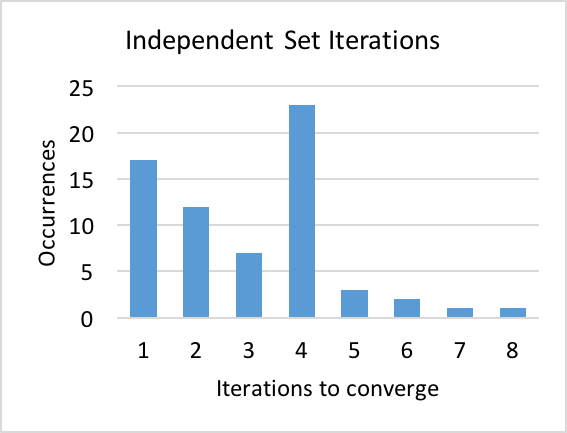
\includegraphics[width=0.3\textwidth]{indset_iters.png}}
\caption{Independent set convergence histogram}\vspace*{-6pt}
\label{fig:indset_conv}
\end{figure}

The proof for the time complexity of Luby's original algorithm
relied on probability theory and changing
the graph node numbers at each iteration \cite{luby1986simple}.
In our algorithm, the number of iterations is bounded by the
length of the longest path in the conflict graph whose nodes have monotonic
quality values.
Although it may be theoretically possible to construct pathological
meshes where this path length grows proportional to the number of elements,
in practice such paths are short.
Figure \ref{fig:indset_conv} shows a histogram of the number of
iterations required to find a maximal independent set during execution
of a typical Omega\_h mesh adaptation.
The algorithm terminates in fewer than ten iterations in all cases,
typically requiring about four iterations.

Finally, note that in line 20 of Algorithm \ref{alg:indset} we
compare graph node global IDs in the case of equal quality values.
Ties could otherwise cause the algorithm to deadlock, and we
prefer a deterministic resolution.
Thus in some cases the output is affected by the global ID values,
however this does not mean it is ordering-dependent because
we update global ID values in a way that is independent
of the local ordering of entities.

\subsubsection{Ghosting for Set Selection}

For distributed memory machines, we implement MPI parallelism
with the help of a generalized ``migration" mechanism.
Migration redistributes the copies of the mesh entities
across MPI ranks \cite{ibanez2015pumi}.
Each MPI rank specifies which entities it requires in the new
partition, using references to entities in the existing
partition.
Multiple MPI ranks may request the same mesh entity, which
is the underlying mechanism to support ghost layers,
since even mesh elements may be requested by multiple ranks.
By using MPI 3.0 features including neighborhood collectives
\cite{hoefler2012optimization}
and graph communicators \cite{hoefler2011scalable},
we developed a scalable migration mechanism.

Our mesh is typically distributed such that each element
is copied to a single MPI rank, and that MPI rank also receives
copies of all entities in the element's boundary.
We call this an element-based partition.
A ghosted partition is constructed
from an element-based partition by having all MPI ranks request
all elements adjacent to the vertices which they had copies
of in the old partition, and the entities bounding those elements.

A ghosted partition has the useful property that every owned entity
(not just elements, but vertices and edges also) has local copies
of all its adjacent entities.
All operations centered around a key entity which read information
from one-level adjacent entities and write information to the
key entity can now be parallelized easily.
Every MPI rank performs the local operation around the key entities
that it owns, and then the information written to the key entities
is communicated from owned copies to all other copies.
For example, the worst element quality resulting from splitting an
edge can be evaluated locally by the MPI rank owning that edge
(because all surrounding element information is available)
and then communicated to the MPI ranks that have copies of that edge
with incomplete surrounding information.

\begin{figure}[t]\vspace*{4pt}
\centerline{
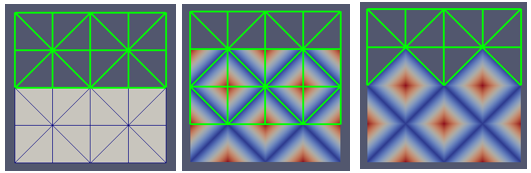
\includegraphics[width=0.5\textwidth]{mpi_indset.png}}
\caption{Steps to distributed adapt: (left) non-ghosted partitions (mid)
add ghost layers, compute independent set (right)
trim away non-owned ghosts}\vspace*{-6pt}
\label{fig:mpi_indset}
\end{figure}

During each adaptation pass, we do what is possible without a ghost
layer first. Typically, this means measuring edge lengths and determining
whether any of them are too long or two short.
Then a ghost layer is constructed and possible operations are evaluated
as described above and an independent set is chosen as described in
Section \ref{sec:indset}.
Once an independent set has been chosen, we return to an element-based
partitioning, but one which is altered such that cavities in the independent
set reside on one MPI rank.
At that point, the code can proceed to apply the cavity modifications
and produce a new local mesh structure without further communication
because shared entities are not modified.
Figure \ref{fig:mpi_indset} illustrates this process at a simple partition boundary,
in the case of selecting which mesh vertices ought to be collapsed.

The tracking of parallel connectivity in our code is based first on global
IDs for the entities.
By the definition of our partitioning, new cavity entities are only created
inside the MPI rank which owns the cavity, so we assign their ownership
to that rank.
We can also take the intersection of entities that stayed the same
(not in cavities) and are owned.
Together these numbers give a count of how many entities in the new mesh are owned
by the local MPI rank.
A simple \texttt{MPI\_Exscan} function call converts local counts into
global numbers for owned copies.
There are still non-owned copies which do not know their global ID, but they
are by definition entities which stayed the same, so we can use the
communication instruments of the old mesh to synchronize their IDs.

Combined with the independent set selection mechanism, this results
in a mesh adaptation method which is unaffected by partition boundaries,
in the sense that the decision process of what modifications to apply
is not influenced by the partition.
The resulting algorithm is also deterministic,
in that its output is the same regardless of the order of
execution of shared memory threads and MPI processes.
Its output is independent
of ordering so long as global IDs are independent of ordering.
Most other parallel adaptation implementations that we know of explicitly
consider interior modifications first, followed by a repartitioning that
allows consideration and modification of the near-boundary mesh
\cite{loseille2015parallel,de1999parallel}, making them
partitioning-dependent.

\section{Determinism}
\label{sec:determinism}

Discuss things done by Omega\_h to achieve
determinism on heterogeneous architectures.

\subsection{Adjacency Inversion}

The key algorithms Ben and I came up with go here.

\subsection{Order-Independent Sums}

%%% Local Variables:
%%% mode: latex
%%% TeX-master: t
%%% End:

